% +------------------------------------------------------------------------+
% | Reference manual page: HalfedgeDS.tex
% +------------------------------------------------------------------------+
% | 22.03.1999   Lutz Kettner
% | Package: HalfedgeDS
% | 
\RCSdef{\RCSHalfedgeDSRev}{$Revision$}
\RCSdefDate{\RCSHalfedgeDSDate}{$Date$}
% +------------------------------------------------------------------------+

\ccRefPageBegin

%%RefPage: end of header, begin of main body
% +------------------------------------------------------------------------+


\begin{ccRefConcept}{HalfedgeDS<Traits,Items,Alloc>}
\ccRefLabel{HalfedgeDS}
%\def\ccPureClassTemplateName{HalfedgeDS<Traits,Items,Alloc>}

\ccCreationVariable{hds}
\ccTagFullDeclarations

% +-----------------------------------+
\ccHeading{Release Note}

Beginning with \cgal\ R2.3, this package has a new design.  The old
design is still available for backwards compatibility and to support
older compiler, such as MSVC++6.0. However its use is deprecated and
the manual pages are not converted into this new manual
format. Instead, see its old documentation in the manual of 
deprecated packages.  The two designs are not interchangeable.

% +-----------------------------------+
\ccDefinition
  
The concept of a halfedge data structure (abbreviated as \ccc{HalfedgeDS}, or
\ccc{HDS} for template parameters) defines an edge-centered data structure
capable of maintaining incidence informations of vertices, edges, and
faces, for example for planar maps or polyhedral surfaces. It is a
combinatorial data structure, geometric interpretation is added by
classes built on top of the halfedge data structure.

The data structure defined here is known as the
FE-structure~\cite{w-ebdss-85}, as
halfedges~\cite{m-ism-88,cgal:bfh-mgedm-95} or as the doubly connected edge
list (DCEL)~\cite{bkos-cgaa-97}, although the original reference for
the DCEL~\cite{mp-fitcp-78} describes a different data structure. The
halfedge data structure can also be seen as one of the variants of the
quad-edge data structure~\cite{gs-pmgsc-85}. In general, the quad-edge
data can represent non-orientable 2-manifolds, but the variant here is
restricted to orientable 2-manifolds only. An overview and comparison
of these different data structures together with a thorough
description of the design implemented here can be found
in~\cite{k-ugpdd-99}.

Each edge is represented by two halfedges with opposite orientations.
Each halfedge can store a reference to an incident face and an
incident vertex.  For each face and each vertex an incident halfedge
is stored.  Reduced variants of the halfedge data structure can omit
some of these incidences, for example the reference to halfedges in
vertices or the storage of vertices at all. See 
Figure~\ccTexHtml{\ref{figureOptionalMethods}}{}\begin{ccHtmlOnly}
  <A HREF="Concept_HalfedgeDS.html#figureOptionalMethods"><IMG 
  SRC="cc_ref_up_arrow.gif" ALT="reference arrow" WIDTH="10" HEIGHT="10"></A>
\end{ccHtmlOnly}
for the incidences, the mandatory and optional member functions
possible for vertices, halfedges, and faces.

\begin{ccTexOnly}
    \begin{figure}[bht]
        \begin{center}
          \parbox{\textwidth}{%
              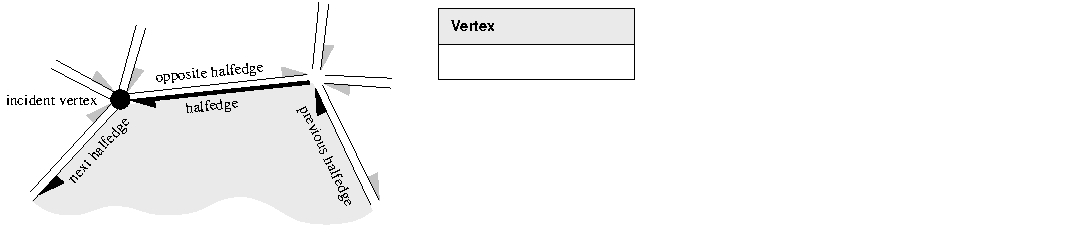
\includegraphics[width=\textwidth]{fig/hds_optional.ips}%
          }
        \end{center}
        \caption{The three classes \protect\ccc{Vertex}, 
          \protect\ccc{Halfedge}, and 
          \protect\ccc{Face} of the halfedge data structure. Member
          functions with shaded background are mandatory. The others
          are optionally supported.}
        \label{figureOptionalMethods}
    \end{figure}
\end{ccTexOnly}

\begin{ccHtmlOnly}
    <CENTER>
    <A NAME="figureOptionalMethods">
    <A HREF="./hds_optional.gif">
        <img src="./hds_optional_small.gif" 
             alt="Class Diagram"></A><BR>
    <A HREF="./hds_optional.gif">Figure:</A>
    The three classes <I>Vertex</I>, <I>Halfedge</I>, and 
          <I>Face</I> of the halfedge data structure. Member
          functions with shaded background are mandatory. The others
          are optionally supported.
    </CENTER>
\end{ccHtmlOnly}

A \ccRefName\ organizes the internal storage of its items.  Examples
are a list-based or a vector-based storage. The \ccRefName\ exhibits
most of the characteristics of the container class used internally,
for example the iterator category. A vector resizes
automatically when a new item exceeds the reserved space. Since
resizing is an expensive operation for a \ccRefName\ in general and
only possible in a well defined state of the data structure (no
dangling handles), it must be called explicitly in advance for a
\ccRefName\ before inserting new items beyond the current capacity.
Classes built on top of a \ccRefName\ are advised to call the
\ccc{reserve()} member function before creating new items.

% +-----------------------------------+
\ccParameters

A \ccRefName\ is a class template and will be used as argument for
other class templates, for example \ccc{CGAL::Polyhedron_3}. The
template parameters to instantiate the \ccRefName\ will be provided by
this other class template. Therefore, the three template parameters
and their meaning are mandatory. We distinguish between the template
\ccRefName\ and an instantiation of it.

\ccc{Traits} is a traits class that will be passed to the 
item types in \ccc{Items}. It will not be used in \ccRefName\
itself. \ccc{Items} is a model of the \ccc{HalfedgeDSItems} concept.
\ccc{Alloc} is a standard allocator that fulfills all requirements 
of allocators for \stl\ container classes. The  \ccc{rebind}
mechanism from \ccc{Alloc} will be used to create appropriate 
allocators internally. A default argument is mandatory for
\ccc{Alloc}, for example, the macro \ccc{CGAL_ALLOCATOR(int)}
from the \ccc{<CGAL/memory.h>} header file can be used as default
allocator.

% +-----------------------------------+
\ccTypes

\ccTwo{HalfedgeDS<Traits,Items,Alloc>:: Halfedge_iterator}{}

\ccNestedType{Traits}{traits class.}
\ccGlue
\ccNestedType{Items}{model of \ccc{HalfedgeDSItems} concept.}

\ccNestedType{size_type}{size type.}
\ccGlue
\ccNestedType{difference_type}{difference type.}
\ccGlue
\ccNestedType{iterator_category}{iterator category for all iterators.}
\ccGlue
\ccNestedType{allocator_type}{allocator type \ccc{Alloc}.}


\ccNestedType{Vertex}{model of \ccc{HalfedgeDSVertex} concept.}
\ccGlue
\ccNestedType{Halfedge}{model of \ccc{HalfedgeDSHalfedge} concept.}
\ccGlue
\ccNestedType{Face}{model of \ccc{HalfedgeDSFace} concept.}

The following handles and iterators have appropriate non-mutable
counterparts, i.e., \ccc{const_handle} and \ccc{const_iterator}. The
mutable types are assignable to their non-mutable counterparts. The
iterators are assignable to the respective handle types. Wherever the
handles appear in function parameter lists, the corresponding
iterators can be used as well. {\bf Note:} The handle types must have
a default constructor that creates a unique and always the same handle
value. It will be used in analogy to \ccc{NULL} for pointers.

\ccNestedType{Vertex_handle}{handle to vertex.}
\ccGlue
\ccNestedType{Halfedge_handle}{handle to halfedge.}
\ccGlue
\ccNestedType{Face_handle}{handle to face.}

\ccNestedType{Vertex_iterator}{iterator over all vertices.}
\ccGlue
\ccNestedType{Halfedge_iterator}{iterator over all halfedges.}
\ccGlue
\ccNestedType{Face_iterator}{iterator over all faces.}

% +-----------------------------------+
\begin{ccAdvanced}
\ccHeading{Types for Tagging Optional Features}

\ccTwo{HalfedgeDS<Traits,Items,Alloc>:: Supports_vertex_halfedge}{}

The following types are equal to either \ccStyle{CGAL::Tag_true} or
\ccStyle{CGAL::Tag_false}, depending on whether the named feature is
supported or not.
\newpage

\ccNestedType{Supports_vertex_halfedge}{\ccc{Vertex::halfedge()}.}
\ccGlue
\ccNestedType{Supports_halfedge_prev}{\ccc{Halfedge::prev()}.}
\ccGlue
\ccNestedType{Supports_halfedge_vertex}{\ccc{Halfedge::vertex()}.}
\ccGlue
\ccNestedType{Supports_halfedge_face}{\ccc{Halfedge::face()}.}
\ccGlue
\ccNestedType{Supports_face_halfedge}{\ccc{Face::halfedge()}.}
\ccGlue
\ccNestedType{Supports_removal}{removal of individual elements.}

The following dependencies among these options must be regarded:

Vertices are supported $\Longleftrightarrow$
\ccc{Supports_halfedge_vertex} $\equiv$ \ccc{CGAL::Tag_true}.
\\
Faces are supported $\Longleftrightarrow$
\ccc{Supports_halfedge_face} $\equiv$ \ccc{CGAL::Tag_true}.
\\
\ccc{Supports_vertex_halfedge} $\equiv$ \ccc{CGAL::Tag_true} $\Longrightarrow$
\ccc{Supports_halfedge_vertex} $\equiv$ \ccc{CGAL::Tag_true}.
\\
\ccc{Supports_vertex_point} $\equiv$ \ccc{CGAL::Tag_true} $\Longrightarrow$
\ccc{Supports_halfedge_vertex} $\equiv$ \ccc{CGAL::Tag_true}.
\\
\ccc{Supports_face_halfedge} $\equiv$ \ccc{CGAL::Tag_true} $\Longrightarrow$
\ccc{Supports_halfedge_face} $\equiv$ \ccc{CGAL::Tag_true}.


\end{ccAdvanced}

% +-----------------------------------+
\begin{ccAdvanced}
\ccHeading{Static Member Functions}
\ccThree{static Halfedge_const_handle}{HalfedgeDS::function}{}

When writing an items type, such as a user defined vertex, certain
functions need to create a handle but knowing only a pointer, for
example, the \ccc{this}-pointer. The following static member functions
of \ccRefName\ create such a corresponding handle for an item type
from a pointer. This conversion encapsulates possible adjustments for
hidden data members in the true item type, such as linked-list
pointers. Note that the user provides item types with the
\ccc{Items} template argument, which may differ from the \ccc{Vertex},
\ccc{Halfedge}, and \ccc{Face} types defined in \ccRefName. If they 
differ, they are derived from the user provided item types. We denote the
user item types with \ccc{Vertex_base}, \ccc{Halfedge_base}, and
\ccc{Face_base} in the following. The fully qualified name for 
\ccc{Vertex_base} would be for example -- assuming that the type \ccc{Self}
refers to the instantiated \ccc{HalfedgeDS} --

\mbox{}~~~~~~\ccc{typedef typename Items::template Vertex_wrapper<Self,Traits>
                 Vertex_wrapper;} \\
\mbox{}~~~~~~\ccc{typedef typename Vertex_wrapper::Vertex  Vertex_base;}

Implementing these functions relies on the fundamental assumption that
an iterator (or handle) of the internally used container class can be
constructed from a pointer of a contained item only. This is true and
controlled by us for \ccc{CGAL::In_place_list}. It is true for the
\ccc{std::vector} of major \stl\ distributions, but not necessarily 
guaranteed. We might switch to an internal implementation if need
arises.

\ccFunction{static Vertex_handle 
  HalfedgeDS::vertex_handle( Vertex_base* v);}{}
\ccGlue
\ccFunction{static Vertex_const_handle 
  HalfedgeDS::vertex_handle( const Vertex_base* v);}{}

\ccFunction{static Halfedge_handle 
  HalfedgeDS::halfedge_handle( Halfedge_base* h);}{}
\ccGlue
\ccFunction{static Halfedge_const_handle 
  HalfedgeDS::halfedge_handle( const Halfedge_base* h);}{}

\ccFunction{static Face_handle 
  HalfedgeDS::face_handle( Face_base* f);}{}
\ccGlue
\ccFunction{static Face_const_handle 
  HalfedgeDS::face_handle( const Face_items* f);}{}

\end{ccAdvanced}

\newpage
% +-----------------------------------+
\ccCreation
\ccThree{HalfedgeDS<Traits,Items,Alloc>& }{functionfoo}{}
\ccThreeToTwo

\ccConstructor{HalfedgeDS();}{empty halfedge data structure.}

\ccConstructor{HalfedgeDS( size_type v, size_type h, size_type f);}
    {storage reserved for $v$ vertices, $h$ halfedges, and $f$ faces.}

\ccTagDefaults
\ccConstructor{HalfedgeDS( const HalfedgeDS<Traits,Items,Alloc>& hds2);}
    {copy constructor. \ccPrecond \ccc{hds2} contains no dangling handles.}

\ccMethod{HalfedgeDS<Traits,Items,Alloc>& 
          operator=( const HalfedgeDS<Traits,Items,Alloc>& hds2);}
    {assignment operator. \ccPrecond \ccc{hds2} contains no dangling handles.}

\ccMethod{void reserve( size_type v, size_type h, size_type f);}
    {reserves storage for $v$ vertices, $h$ halfedges, and $f$ faces.
     If all capacities are already greater or equal than the requested sizes
     nothing happens. Otherwise, \ccVar\ will be resized and all handles, 
     iterators and circulators invalidate. \ccPrecond If resizing is
     necessary \ccVar\ contains no dangling handles.}


% +-----------------------------------+
\ccHeading{Access Member Functions}
\ccThree{Halfedge_iterator}{hds.capacity_of_halfedges();}{}

\ccMethod{Size size_of_vertices() const;}{number of vertices.}
\ccGlue
\ccMethod{Size size_of_halfedges() const;}{number of halfedges.}
\ccGlue
\ccMethod{Size size_of_faces() const;}{number of faces.}
\ccGlue
\ccMethod{Size capacity_of_vertices() const;}{space reserved for vertices.}
\ccGlue
\ccMethod{Size capacity_of_halfedges() const;}{space reserved for halfedges.}
\ccGlue
\ccMethod{Size capacity_of_faces() const;}{space reserved for faces.}
\ccGlue
\ccMethod{size_t bytes() const;}{bytes used for \ccVar.}
\ccGlue
\ccMethod{size_t bytes_reserved() const;}{bytes reserved for \ccVar.}

\ccMethod{allocator_type get_allocator() const;}{allocator object.}

The following member functions return the non-mutable iterator if
\ccVar\ is declared const.

\ccMethod{Vertex_iterator    vertices_begin();}{iterator over all vertices.}
\ccGlue
\ccMethod{Vertex_iterator    vertices_end();}{}
\ccGlue
\ccMethod{Halfedge_iterator  halfedges_begin();}{iterator over all halfedges}
\ccGlue
\ccMethod{Halfedge_iterator  halfedges_end();}{}
\ccGlue
\ccMethod{Face_iterator     faces_begin();}{iterator over all faces.}
\ccGlue
\ccMethod{Face_iterator     faces_end();}{}

% +-----------------------------------+
\ccHeading{Insertion}
\ccTagFullDeclarations

Note that the vertex-related and the face-related member functions may
not be provided for a \ccRefName\ that does not support vertices or
faces respectively.

\ccMethod{Vertex_handle vertices_push_back( const Vertex& v);}
    {appends a copy of $v$ to \ccc{hds}. Returns a handle of the new vertex.}

\ccMethod{Halfedge_handle edges_push_back( const Halfedge& h, 
                                           const Halfedge& g);}
    {appends a copy of $h$ and a copy of $g$ to \ccc{hds} and makes them
     opposite to each other. Returns a handle of the copy of $h$.}

\ccMethod{Halfedge_handle edges_push_back( const Halfedge& h);}
    {appends a copy of $h$ and a copy of $h->opposite()$ to \ccc{hds} and 
     makes them opposite to each other. Returns a handle of the copy of $h$.
     \ccPrecond \ccc{h->opposite()} denotes a halfedge.}

\ccMethod{Face_handle faces_push_back( const Face& f);}
    {appends a copy of $f$ to \ccc{hds}. Returns a handle of the new face.}


% +-----------------------------------+
\ccHeading{Removal}
\ccThree{Halfe}{dge_iteratorhds.capacity_of_halfedges();}{}

Erasing single elements is optional and indicated with the type tag
\ccc{Supports_removal}. The \ccc{pop_back} and the \ccc{clear} member 
functions are mandatory. If vertices or faces are not supported 
for a \ccRefName\ the \ccc{pop_back} and the \ccc{clear} member 
functions must be provided as null operations.

\ccMethod{void vertices_pop_front();}{
    removes the first vertex if vertices are supported and
    \ccc{Supports_removal} $\equiv$ \ccc{CGAL::Tag_true}.}

\ccMethod{void vertices_pop_back();}{
    removes the last vertex.}

\ccMethod{void vertices_erase( Vertex_handle v);}{
    removes the vertex $v$ if vertices are supported and
    \ccc{Supports_removal} $\equiv$ \ccc{CGAL::Tag_true}.}

\ccMethod{void vertices_erase( Vertex_handle first, Vertex_handle last);}{
    removes the range of vertices $[\ccc{first},\ccc{last})$ if vertices 
    are supported and \ccc{Supports_removal} $\equiv$ \ccc{CGAL::Tag_true}.}

\ccMethod{void edges_pop_front();}{
    removes the first two halfedges if
    \ccc{Supports_removal} $\equiv$ \ccc{CGAL::Tag_true}.}

\ccMethod{void edges_pop_back();}{
    removes the last two halfedges.}

\ccMethod{void edges_erase( Halfedge_handle h);}{
    removes the pair of halfedges $h$ and \ccc{h->opposite()}
    if \ccc{Supports_removal} $\equiv$ \ccc{CGAL::Tag_true}.}

\ccMethod{void edges_erase( Halfedge_handle first, Halfedge_handle last);}{
    removes the range of edges $[\ccc{first},\ccc{last})$ if
    \ccc{Supports_removal} $\equiv$ \ccc{CGAL::Tag_true}.}

\ccMethod{void faces_pop_front();}{
    removes the first face if faces are supported and
    \ccc{Supports_removal} $\equiv$ \ccc{CGAL::Tag_true}.}

\ccMethod{void faces_pop_back();}{
    removes the last face.}

\ccMethod{void faces_erase( Face_handle f);}{
    removes the face $f$ if faces are supported and
    \ccc{Supports_removal} $\equiv$ \ccc{CGAL::Tag_true}.}

\ccMethod{void faces_erase( Face_handle first, Face_handle last);}{
    removes the range of faces $[\ccc{first},\ccc{last})$ if faces are 
    supported and \ccc{Supports_removal} $\equiv$ \ccc{CGAL::Tag_true}.}

\ccMethod{void vertices_clear();}{removes all vertices.}
\ccGlue
\ccMethod{void edges_clear();}{removes all halfedges.}
\ccGlue
\ccMethod{void faces_clear();}{removes all faces.}

\ccMethod{void clear();}{removes all elements.}


% +-----------------------------------+
\begin{ccAdvanced}
\vspace*{-2mm}
\ccHeading{Operations with Border Halfedges}
  
The following notion of {\em border halfedges\/} is particular useful
where the halfedge data structure is used to model surfaces with
boundary, i.e., surfaces with missing faces or open regions. Halfedges
incident to an open region are called {\em border halfedges}. A
halfedge is a {\em border edge\/} if the halfedge itself or its
opposite halfedge is a border halfedge. The only requirement to work
with border halfedges is that the
\ccc{Halfedge} class provides a member function \ccc{is_border()}
returning a \ccc{bool}. Usually, the halfedge data structure
supports faces and the value of the default constructor of the face
handle will indicate a border halfedge, but this may not be the only
possibility. The \ccc{is_border()} predicate divides the edges into
two classes, the border edges and the non-border edges. The
following normalization reorganizes the sequential storage of the
edges such that the non-border edges precede the border edges, and
that for each border edge the latter of the two halfedges is a
border halfedge (the first one might be a border halfedge too). The
normalization stores the number of border halfedges, as well as the
halfedge iterator where the border edges start at, within the
halfedge data structure.  These values will be invalid after further
halfedge insertions or removals and changes in the border status of 
a halfedge. There is no automatic update required.

\ccThree{Halfedge_iterator}{hds.size_of;}{}

\ccMethod{void   normalize_border();}
    {sorts halfedges such that the non-border edges precede the
     border edges. For each border edge that is incident to a face,
     the halfedge iterator will reference the halfedge incident to the
     face right before the halfedge incident to the open region.}

\ccMethod{Size size_of_border_halfedges() const;}
    {number of border halfedges. An edge with no incident face
      counts as two border halfedges.
    \ccPrecond \ccc{normalize_border()} has been called and no
    halfedge insertion or removal and no change in border
    status of the halfedges have occurred since then.}

\ccMethod{Size size_of_border_edges() const;}
    {number of border edges. If \ccc{size_of_border_edges()} is equal
    to \ccc{size_of_border_halfedges()} all border edges are incident to
    a face on one side and to an open region on the other side.
    \ccPrecond \ccc{normalize_border()} has been called and no
    halfedge insertion or removal and no change in border
    status of the halfedges have occurred since then.}

\ccMethod{Halfedge_iterator  border_halfedges_begin();}
    {halfedge iterator starting with the border edges. The range
      [\ccStyle{halfedges_begin(), border_halfedges_begin()}) denotes
    all non-border edges. The range
    [\ccStyle{border_halfedges_begin(), halfedges_end()}) denotes all
    border edges.
    \ccPrecond \ccc{normalize_border()} has been called and no
    halfedge insertion or removal and no change in border
    status of the halfedges have occurred since then.}

\vspace*{-4mm}
\end{ccAdvanced}


% +-----------------------------------+
\ccHasModels

\ccRefIdfierPage{CGAL::HalfedgeDS_default}\\
\ccRefIdfierPage{CGAL::HalfedgeDS_list}\\
\ccRefIdfierPage{CGAL::HalfedgeDS_vector}

% +-----------------------------------+
\ccSeeAlso

\ccRefConceptPage{HalfedgeDSItems}\\
\ccRefIdfierPage{CGAL::Polyhedron_3<Traits>}\\
\ccRefIdfierPage{CGAL::HalfedgeDS_vertex_base<Refs>}\\
\ccRefIdfierPage{CGAL::HalfedgeDS_halfedge_base<Refs>}\\
\ccRefIdfierPage{CGAL::HalfedgeDS_face_base<Refs>}\\
\ccRefIdfierPage{CGAL::HalfedgeDS_items_decorator<HDS>}\\
\ccRefIdfierPage{CGAL::HalfedgeDS_decorator<HDS>}\\
\ccRefIdfierPage{CGAL::HalfedgeDS_const_decorator<HDS>}

% +-----------------------------------+
\ccImplementation

Classes parameterized with a halfedge data structure, such as
\ccc{CGAL::Polyhedron_3}, need to declare a class template as one of its
template parameters for the \ccRefName. For compilers not supporting
this (i.e.~the flag \ccc{CGAL_CFG_NO_TMPL_IN_TMPL_PARAM} is set), the
following workaround is required, which defines a \ccRefName\ as a
normal class that contains a member class template named \ccc{HDS},
which is the actual halfedge data structure as defined here. The
following program fragment illustrates this workaround:

\begin{ccExampleCode}
#ifndef CGAL_CFG_NO_TMPL_IN_TMPL_PARAM
    template <class Traits, class Items, class Alloc> 
    class HalfedgeDS {
    public:
        typedef HalfedgeDS<Traits,Items,Alloc> Self;
        HalfedgeDS_vector(); // constructors
#else
    struct HalfedgeDS {
    template <class Traits, class Items, class Alloc> 
    class HDS {
    public:
        typedef HDS<Traits,Items,Alloc> Self;
        HDS(); // constructors
#endif
        // ... further member functions. Self denotes the HalfedgeDS.
    };
#ifdef CGAL_CFG_NO_TMPL_IN_TMPL_PARAM
    };
#endif
\end{ccExampleCode}

\ccTagDefaults

\end{ccRefConcept}

% +------------------------------------------------------------------------+
%%RefPage: end of main body, begin of footer
\ccRefPageEnd
% EOF
% +------------------------------------------------------------------------+

